\documentclass[12pt, leqno]{article} %% use to set typesize
\input{common}

\usepackage{fontspec}
\usepackage{polyglossia}
\setmonofont{DejaVu Sans Mono}[Scale=MatchLowercase]
\usepackage[outputdir=pdf]{minted}

\providecommand{\tightlist}{%
  \setlength{\itemsep}{0pt}\setlength{\parskip}{0pt}}
\begin{document}



\hdr{2023-03-31}

\section{Optimization essentials}

Last time, we mostly focused on solving systems of nonlinear equations.
Today, we consider optimization problems. The two perspectives are very
complimentary, but we will delve into that further after break.

Recall from your calculus classes the second-order Taylor expansion. If
\(\phi : \mathbb{R}^n \rightarrow \mathbb{R}\) is \(\mathcal{C}^2\)
(i.e.~if it is at least twice continuously differentiable) then we have
the expansion
\[\phi(x+u) = \phi(x) + \phi'(x) u + \frac{1}{2} u^T H_{\phi}(x) u + o(\|u\|^2)\]
where \(\phi'(x) \in \mathbb{R}^{1 \times n}\) is the derivative of
\(\phi\) and \(H_{\phi}\) is the \emph{Hessian matrix} consisting of
second derivatives:
\[(H_\phi)_{ij} = \frac{\partial \phi}{\partial x_i \partial x_j}.\] The
\emph{gradient} \(\nabla \phi(x) = \phi'(x)^T\) is a column vector
(rather than a row vector).

Let's give an illustration comparing a function
\(\phi_{\mathrm{ex}} : \mathbb{R}^2 \rightarrow \mathbb{R}\) to the
first and second-order Taylor expansions about some point \(x_0\). To do
this, we will need the gradient and the Hessian \begin{align*}
  \phi(x) &= -\cos(x_1 + x_2) + \sin(x_2)^2\\
  \nabla \phi(x) &=
  \begin{bmatrix} \sin(x_1 + x_2) \\ \sin(x_1+x_2) + \sin(2x_2) \end{bmatrix} \\
  H_{\phi} &=
  \begin{bmatrix}
  \cos(x_1+x_2) & \cos(x_1+x_2) \\
  \cos(x_1+x_2) & \cos(x_1+x_2) + 2 \cos(2x_2)
  \end{bmatrix}
\end{align*}

\begin{figure}
\begin{center}
  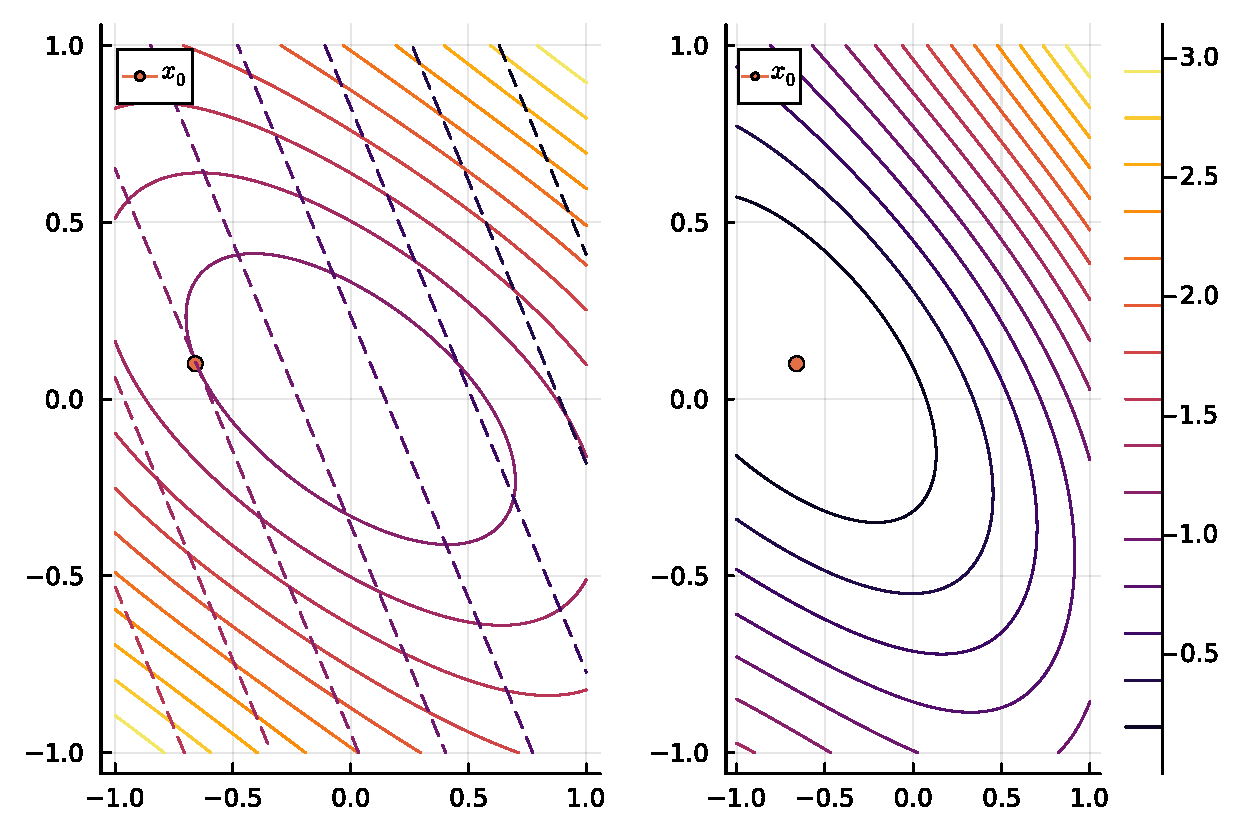
\includegraphics[width=0.8\textwidth]{fig/2023-03-31-taylor1.pdf}
\end{center}
\caption{Contour plot of $\phi$ vs first-order Taylor approximation $\hat{\phi}$ (left) and plot of $\phi-\hat{\phi}$ (right).}
\label{fig:taylor1}
\end{figure}

\begin{figure}
\begin{center}
  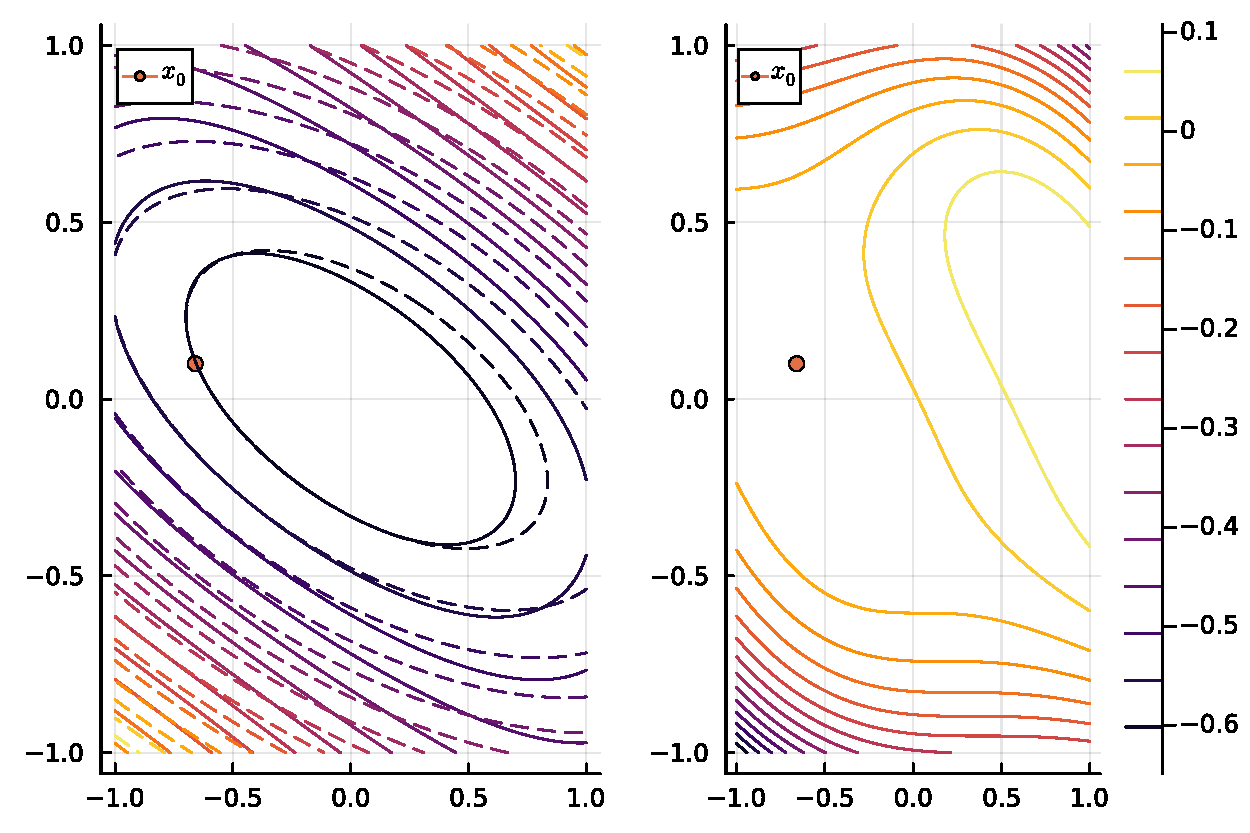
\includegraphics[width=0.8\textwidth]{fig/2023-03-31-taylor2.pdf}
\end{center}
\caption{Contour plot of $\phi$ vs second-order Taylor approximation $\hat{\phi}$ (left) and plot of $\phi-\hat{\phi}$ (right).}
\label{fig:taylor2}
\end{figure}

We compare $\phi$ to first-order and second-order Taylor expansions in
Figures~\ref{fig:taylor1}-\ref{fig:taylor2}.


If \(\nabla \phi(x) \neq 0\) then \(\nabla \phi(x)\) and
\(-\nabla \phi(x)\) are the directions of steepest ascent and descent,
respectively (we will have more to say on this point presently). If
\(\nabla \phi(x) = 0\), then we say \(x\) is a \emph{stationary point}
or \emph{critical point}. The first derivative test says that if \(x\)
minimizes \(\phi\) (and \(\phi\) is differentiable) then the gradient of
\(x\) must be zero; otherwise, there is a ``downhill'' direction, and a
point near \(x\) achieves a smaller function value.

A stationary point does not need to be a local minimizer; it might also
be a maximizer, or a saddle point. The \emph{second} derivative test
says that for a critical point \(x\) to be a (local) minimizer, the
Hessian \(H_{\phi}(x)\) must be at least positive semi-definite. If
\(x\) is a stationary point and \(H_{\phi}\) is strictly positive
definite, then \(x\) must be a local minimizer; in this case, we call
\(x\) a \emph{strong} local minimizer.

One approach to the problem of minimizing \(\phi\) is to run Newton
iteration on the critical point equation \(\nabla \phi(x) = 0\). The
Jacobian of the function \(\nabla \phi(x)\) is simply the Hessian
matrix, so Newton's iteration for finding the critical point is just
\[x_{k+1} = x_k - H_{\phi}(x_k)^{-1} \nabla \phi(x_k).\] We can derive
this in the same way that we derived Newton's iteration for other
nonlinear equations; or we can derive it from finding the critical point
of a quadratic approximation to \(\phi\): \[\hat{\phi}(x_k+p_k) =
  \phi(x_k) + \phi'(x_k) p_k + \frac{1}{2} p_k^T H_{\phi}(x_k) p_k.\]
The critical point occurs for
\(p_k = -H_{\phi}(x_k)^{-2} \nabla \phi(x_k)\); but this critical point
is a strong local minimum iff \(H_{\phi}(x_k)\) is positive definite.

\begin{minted}{julia}
function plot_convergence(ϕ, xs, resids)
    xx = range(-1.0, 1.0, length=100)
    p1 = plot(xx, xx, ϕ, st=:contour)
    plot!([x[1] for x in xs], [x[2] for x in xs], marker=true, label=false)
    p2 = plot(resids[resids .> 0], yscale=:log10, legend=false)
    plot(p1, p2, layout=(1,2))
end
\end{minted}

\begin{minted}{julia}
let
    x = [0.0; 0.5]

    # Newton loop -- plot where we're going
    resids = []
    xs = [copy(x)]

    for k = 1:5

        # Compute the gradient and record the norm
        g = ∇ϕex(x)
        push!(resids, norm(g))

        # Take a Newton step and record the point
        x -= Hϕex(x)\g
        push!(xs, copy(x))

    end

    # Plot the function and the iterates
    plot_convergence((x,y)->ϕex([x; y]), xs, resids)
end
\end{minted}

\begin{figure}
\begin{center}
  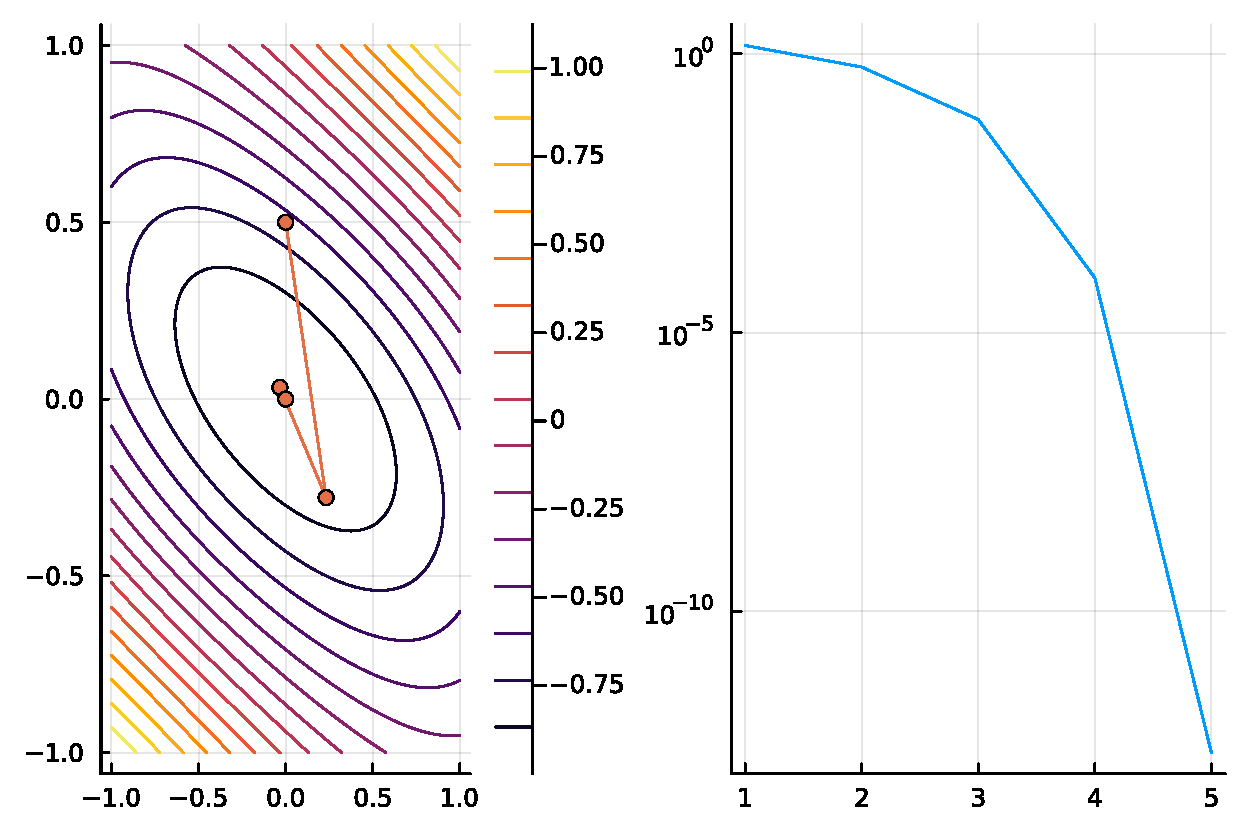
\includegraphics[width=0.8\textwidth]{fig/2023-03-31-newton.pdf}
\end{center}
\caption{Convergence of Newton iteration on example $\phi$.}
\label{fig:newton}
\end{figure}

There are a couple reasons we might want to not just say ``run Newton to
find a critical point'' and call it a day. Three key ones are:

\begin{itemize}
\tightlist
\item
  Computing Hessians can be a bit of a pain.
\item
  We can take advantage of the fact that this is \emph{not} a general
  system of nonlinear equations in devising and analyzing methods.
\item
  If we only seek to solve the critical point equation, we might end up
  finding a maximizer or saddle point as easily as a minimizer.
\end{itemize}

For this reason, we will discuss a different class of iterations, the
(scaled) gradient descent methods and their relatives.

\subsection{Questions}

For all these questions, assume \(\phi\) is twice continuously
differentiable and that the Hessian \(H_{\phi}\) is Lipschitz with
constant \(M\).

\begin{enumerate}
\def\labelenumi{\arabic{enumi}.}
\tightlist
\item
  Change the starting point in the iteration above (e.g.~to the point
  \((0, 0.6)\)). What changes?
\item
  Explain why
  \(\phi(x+u) = \phi(x) + \nabla \phi(x)^T u + \frac{1}{2} u^T H_{\phi}(x+\xi u) u\)
  for some \(\xi \in [0,1]\).
\item
  Argue that
  \(|\phi(x) + \nabla \phi(x)^T u + \frac{1}{2} u^T H_{\phi}(x) u - \phi(x+u)| \leq \frac{M}{2} \|u\|^3\).
\item
  Let \(p\) be a Newton update starting from \(x\), and let
  \(w = \phi(x)-\phi(x+p)\) be the improvement in the function value
  during that Newton step. Show that
  \(\left| w-\frac{1}{2} p^T H_{\phi}(x) p \right| \leq \frac{M}{2} \|p\|^3\).
\end{enumerate}

\section{Gradient descent}

One of the simplest optimization methods is the \emph{steepest descent}
or \emph{gradient descent} method \[x_{k+1} = x_k + \alpha_k p_k\] where
\(\alpha_k\) is a \emph{step size} and \(p_k = -\nabla \phi(x_k)\).

Let's try an example using the test function above. Play with
\(\alpha\). What happens to the convergence?

\begin{minted}{julia}
let
    x = [0.0; 0.5]
    α=0.1

    # Gradient descent loop -- plot where we're going
    resids = []
    xs = [copy(x)]

    for k = 1:100

        # Compute the gradient and record the norm
        g = ∇ϕex(x)
        push!(resids, norm(g))

        # Take a gradient descent step and record the point
        x -= α*g
        push!(xs, copy(x))

    end

    # Plot the function and the iterates
    plot_convergence((x,y)->ϕex([x; y]), xs, resids)
end
\end{minted}

\begin{figure}
\begin{center}
  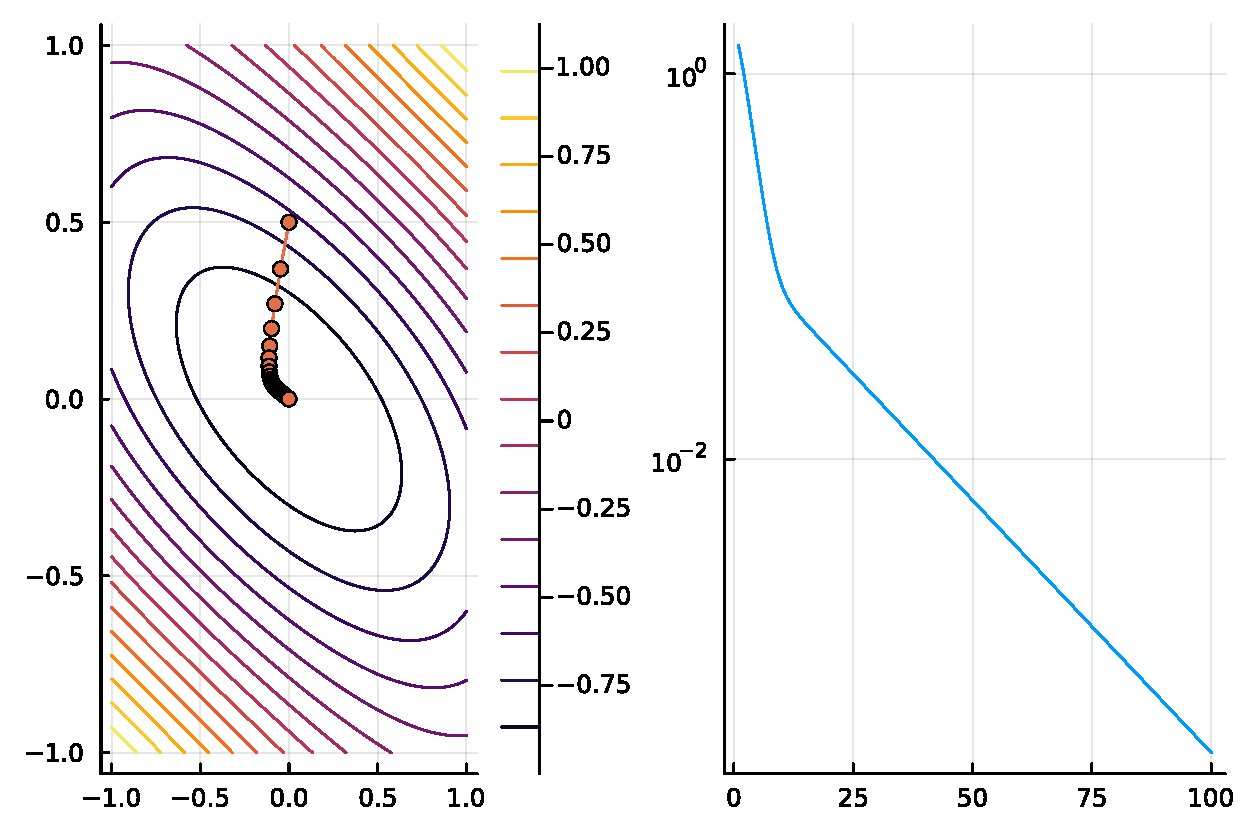
\includegraphics[width=0.8\textwidth]{fig/2023-03-31-gradient.pdf}
\end{center}
\caption{Convergence of gradient descent on example $\phi$.}
\label{fig:gradient}
\end{figure}

To understand the convergence of this method, consider gradient descent
with a fixed step size \(\alpha\) for the quadratic model problem
\[\phi(x) = \frac{1}{2} x^T A x + b^T x + c\] where \(A\) is symmetric
positive definite. We have computed the gradient for a quadratic before:
\[\nabla \phi(x) = Ax + b,\] which gives us the iteration equation
\[x_{k+1} = x_k - \alpha (A x_k + b).\] Subtracting the fixed point
equation \[x_* = x_* - \alpha (A x_* + b)\] yields the error iteration
\[e_{k+1} = (I-\alpha A) e_k.\] If \(\{ \lambda_j \}\) are the
eigenvalues of \(A\), then the eigenvalues of \(I-\alpha A\) are
\(\{ 1-\alpha \lambda_j \}\). The spectral radius of the iteration
matrix is thus \[\min \{ |1-\alpha \lambda_j| \}_j =
  \min \left( |1-\alpha \lambda_{\min}|, |1-\alpha \lambda_{\max}| \right).\]
The iteration converges provided \(\alpha < 1/\lambda_{\max}\), and the
optimal \(\alpha\) is
\[\alpha_* = \frac{2}{\lambda_{\min} + \lambda_{\max}},\] which leads to
the spectral radius
\[1 - \frac{2 \lambda_{\min}}{\lambda_{\min} + \lambda_{\max}} =
  1 - \frac{2}{1 + \kappa(A)}\] where
\(\kappa(A) = \lambda_{\max}/\lambda_{\min}\) is the condition number
for the (symmetric positive definite) matrix \(A\). If \(A\) is
ill-conditioned, then, we are forced to take very small steps to
guarantee convergence, and convergence may be heart breakingly slow. We
will get to the minimum in the long run --- but, then again, in the long
run we all die.

Our example problem is not quadratic, of course. But close to the
minimum at \((0,0)\), it is close enough to quadratic that we get a good
picture of the convergence from the quadratic approximation.

\begin{figure}
\begin{center}
  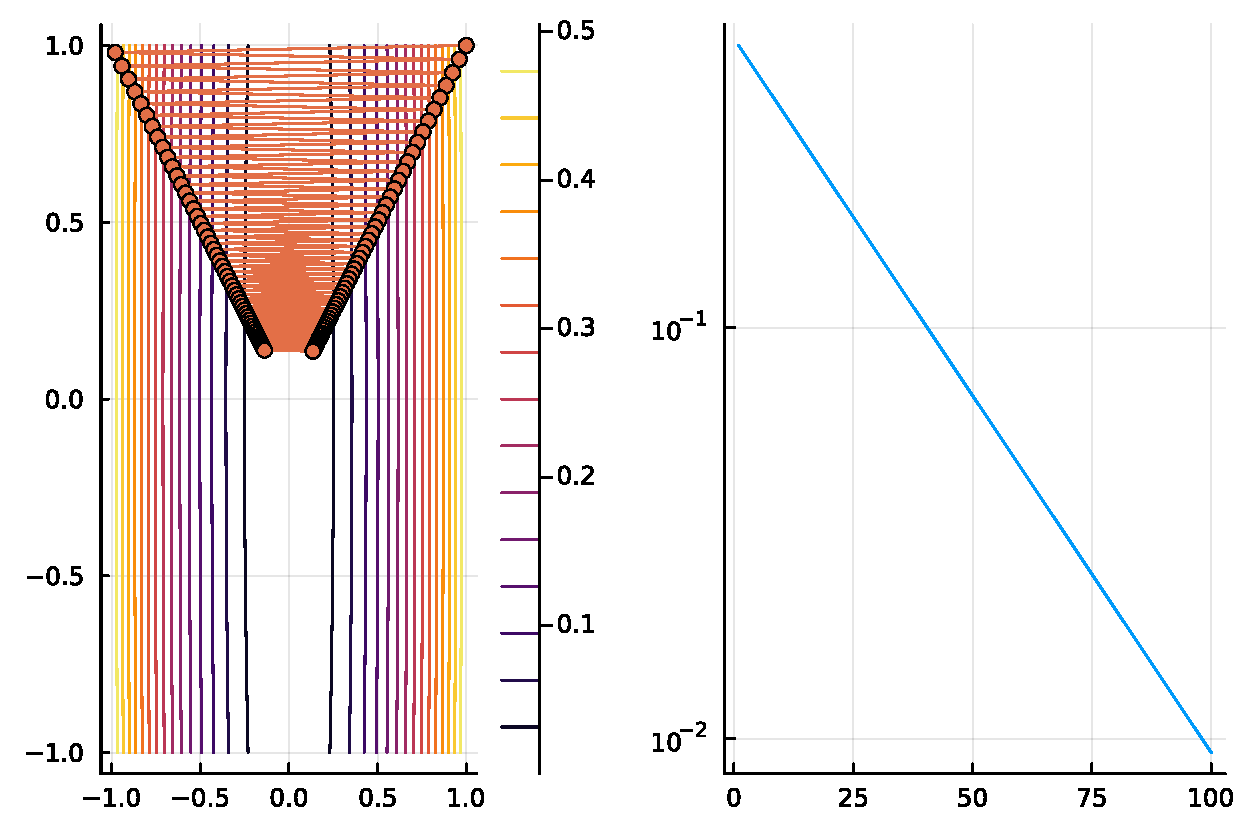
\includegraphics[width=0.8\textwidth]{fig/2023-03-31-gradient-bad.pdf}
\end{center}
\caption{Convergence of gradient descent on an ill-conditioned problem.}
\label{fig:gradient-bad}
\end{figure}

If we take a somewhat less well-conditioned problem, we get a
significantly slower optimal rate of convergence
(Figure~\ref{fig:gradient-bad}).

\begin{minted}{julia}
let
    A = [1.0 0.0; 0.0 1e-2]
    x = [1.0; 1.0]
    λs = eigvals(A)
    α = 2/(λs[1]+λs[2])

    # Steepest descent loop
    xs = [copy(x)]
    resids = []
    for k = 1:100
        x -= α*A*x
        push!(xs, copy(x))
        push!(resids, 0.5*x'*A*x)
    end

    # Plot the function and the iterates
    plot_convergence((x,y)->0.5*[x; y]'*A*[x; y], xs, resids)
end
\end{minted}

The behavior of steepest descent iteration on a quadratic model problem
is indicative of the behavior more generally: if \(x_*\) is a strong
local minimizer of some general nonlinear \(\phi\), then gradient
descent with sufficiently small step size will converge locally to
\(x_*\). But if \(H_{\phi}(x_*)\) is ill-conditioned, then one has to
take small steps, and the rate of convergence can be quite slow.

Not all problems are terrible ill-conditioned, and so in many cases
simple gradient descent algorithms can work quite well. For
ill-conditioned problems, though, we would like to change something
about the algorithm. One approach is to keep the gradient descent
direction and adapt the step size in a clever way; the Barzelei-Borwein
(BB) method and related approaches follow this approach. These
remarkable methods deserve to be better known, but in the interest of
fitting the course into the semester, we will turn instead to the
problem of choosing better directions.

\section{``Steepest'' descent}

At a point \(x\), a direction \(p\) is a \emph{descent} direction for
\(\phi\) if \(\phi'(x) p < 0\). We measure how ``steep'' a descent
direction is by the rate at which the function value decreases if we
move at unit speed in that direction: \(-\phi'(x) p/\|p\|\). If
\(\|\cdot\|\) is the ordinary Euclidean norm on \(\mathbb{R}^n\), we
have that the direction of steepest descent is
\(-\phi'(x)^T/\|\phi'(x)\|\). But what happens if we use a different
norm for measuring distance?

Put differently, consider the problem of maximizing \(-g^T u\) over the
ball \(\|u\| \leq 1\). Then

\begin{itemize}
\tightlist
\item
  Over \(\|u\|_2 \leq 1\), we have \(u = -g/\|g\|\)
\item
  Over \(\|u\|_\infty \leq 1\), we have \(u = -\operatorname{sign}(g)\)
\item
  Over \(\|u\|_1 \leq 1\), we have \(u = -\operatorname{sign}(g_k) e_k\)
  where \(g_k\) is the largest magnitude entry of \(g\).
\end{itemize}

Of course, these are not the only norms out there. In particular, if
\(M\) is a positive definite matrix, then there is an associated inner
product \[\langle x, y \rangle_M = y^* M x\] and an associated Euclidean
norm \[\|x\|_M = \sqrt{x^T M x}.\] Maximizing \(-g^T u / \|u\|_M\) gives
us \(u \propto -M^{-1} g\).

\section{Scaled gradient descent}

The \emph{scaled} gradient descent iteration takes the form
\[x_{k+1} = x_k + \alpha_k p_k, \quad M_k p_k = -\nabla \phi(x_k).\]
where \(\alpha_k\) and \(p_k\) are the step size and direction, as
before, and \(M_k\) is a symmetric positive definite \emph{scaling
matrix}. We can also see this as ordinary steepest descent, but steepest
descent with respect to the adaptively-chosen \(M_k\) Euclidean norms.

Positive definiteness of \(M_k\) guarantees that \(p_k\) is a
\emph{descent direction}, i.e. \[\phi'(x_k) p_k = \nabla \phi(x_k)^T p_k
  = -\nabla \phi(x_k)^T M_k^{-1} \nabla \phi(x_k) < 0;\] this in turn
guarantees that if \(\alpha_k\) is sufficiently small, \(\phi(x_{k+1})\)
will be less than \(\phi(x_k)\) --- unless \(\phi(x_k)\) is a stationary
point (i.e.~\(\nabla \phi(x_k) = 0\)).

How does scaling improve on simple gradient descent? Consider again the
quadratic model problem \[\nabla \phi(x) = Ax + b,\] and let \(M\) and
\(\alpha\) be fixed. With a little work, we derive the error iteration
\[e_{k+1} = (I-\alpha MA) e_k\] If \(\alpha M = A^{-1}\), the iteration
converges in a single step! Going beyond the quadratic model problem, if
\(x_*\) was a known strong local minimizer, we could use
\(M_k = H_{\phi}(x_*)\) -- which will give us superlinear convergence.

\begin{figure}
\begin{center}
  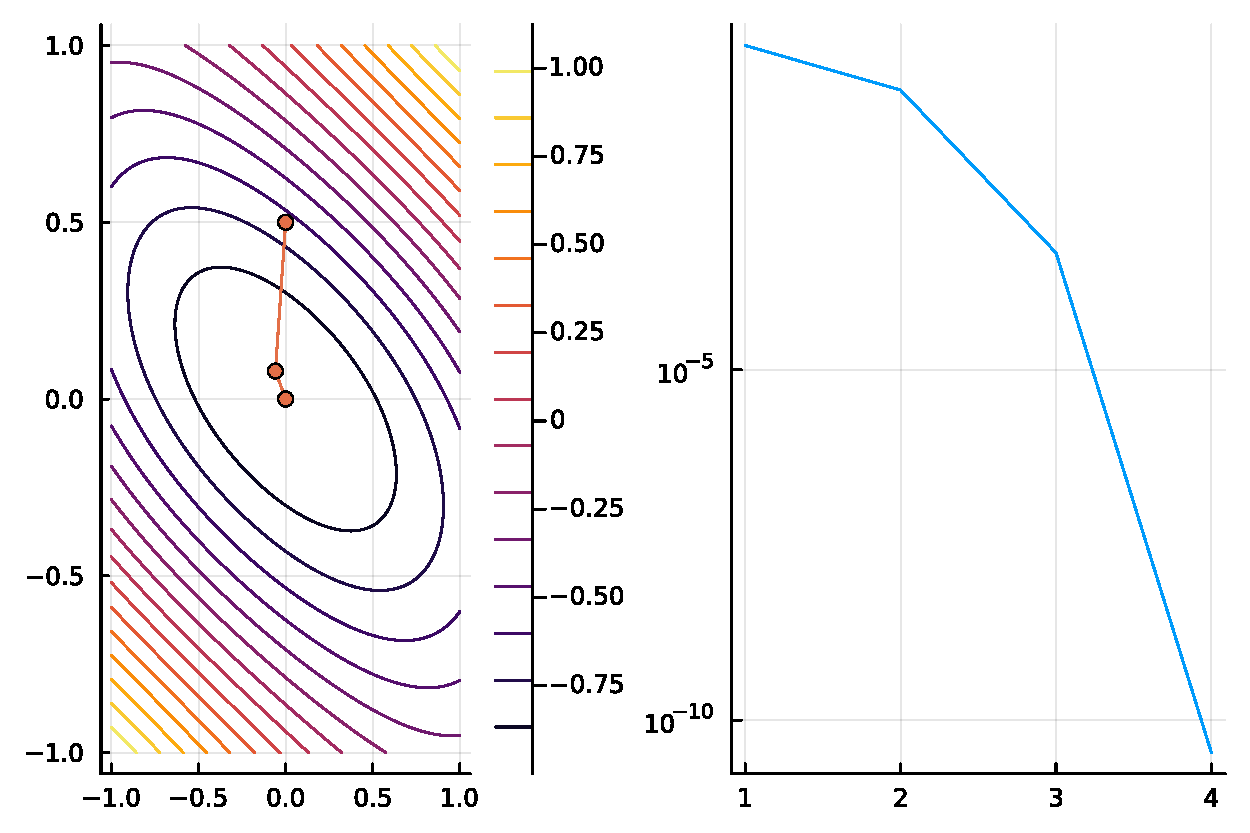
\includegraphics[width=0.8\textwidth]{fig/2023-03-31-gradient-scaled.pdf}
\end{center}
\caption{Convergence of scaled gradient descent.}
\label{fig:gradient-scaled}
\end{figure}

The convergence of the scaled gradient descent iteration below is
shown in Figure~\ref{fig:gradient-scaled}.

\begin{minted}{julia}
let
    x = [0.0; 0.5]
    α=1.0

    # Scaled steepest descent loop -- plot where we're going
    resids = []
    xs = [copy(x)]
    M = Hϕex([0; 0])

    for k = 1:5

        # Compute the gradient and record the norm
        g = M\∇ϕex(x)
        push!(resids, norm(g))

        # Take a gradient descent step and record the point
        x -= α*g
        push!(xs, copy(x))

    end

    # Plot the function and the iterates
    plot_convergence((x,y)->ϕex([x; y]), xs, resids)
end
\end{minted}

In general, we cannot scale with \(H_{\phi}(x_*)\), since we don't know
the location of \(x_*\)! But if \(H_{\phi}(x_k)\) is positive definite,
we might choose \(M_k = H_{\phi}(x_k)\) --- which would correspond to a
Newton step. Of course, \(H_{\phi}(x_k)\) does not have to be positive
definite everywhere! Thus, most minimization codes based on Newton
scaling use \(M_k = H_{\phi}(x_k)\) when it is positive definite, and
otherwise use some modification. One possible modification is to choose
a diagonal shift \(M_k = H_{\phi}(x_k) + \beta I\) where \(\beta\) is
sufficiently large to guarantee positive definiteness. Another common
approach is to compute a \emph{modified Cholesky} factorization of
\(H_{\phi}(x_k)\). The modified Cholesky algorithm looks like ordinary
Cholesky, and is identical to ordinary Cholesky when \(H_{\phi}(x_k)\)
is positive definite. But rather than stopping when it encounters a
negative diagonal in a Schur complement, the modified Cholesky approach
replaces that element with something else and proceeds.

\subsection{Questions}

Suppose \(\phi\) is a \(C^2\) function and \(H_{\phi}\) is Lipschitz
with constant \(M\). Let \(x_*\) be a strong local minimizer for
\(\phi\) and consider the scaled steepest descent iteration
\[x_{k+1} = x_k - H_{\phi}(x_*)^{-1} \nabla \phi(x_k)\] Subtract off the
fixed point equation to get
\[e_{k+1} = e_k - H_{\phi}(x_*)^{-1} \left( \nabla \phi(x_*+e_k) - \nabla \phi(x_*) \right)\]
Conclude that for some \(\xi \in [0,1]\),
\[\|e_{k+1}\| \leq \| H_{\phi}(x_*)^{-1} \left(H_{\phi}(x_*) - H_{\phi}(x_* + \xi e_k)\right) e_k \|,\]
which implies under the Lipschitz assumption that
\[\|e_{k+1}\| \leq \|H_{\phi}(x_*)^{-1}\| M \|e_k\|^2.\] Therefore, the
iteration converges quadratically for good enough initial guesses. Can
you also give a condition on \(\|e_0\|\) that guarantees an initial
guess is ``good enough''?


\end{document}
